\subsection{Preventivo a finire completo} 
Nel preventivo riportiamo la spesa totale che il committente dovrà affrontare, derivata dal totale delle ore rendicontate e preventivate nelle fasi di progettazione, sviluppo, e collaudo.

\subsubsection{Divisione oraria complessiva} 
La seguente tabella rappresenta la distribuzione oraria dei ruoli per ogni componente del gruppo:
{
	\rowcolors{2}{\evenRowColor}{\oddRowColor}
\renewcommand{\arraystretch}{2}
\begin{longtable}[h!] { C{3.5cm} C{1cm} C{1cm} C{1cm} C{1cm} C{1cm} C{1cm} C{2cm}}
\caption{Tabella della divisione oraria complessiva}	\\
\rowcolor{\primaryColor}

\textcolor{\secondaryColor}{\textbf{Membro del gruppo}} & 
\textcolor{\secondaryColor}{\textbf{RE}} & 
\textcolor{\secondaryColor}{\textbf{AM}} & 
\textcolor{\secondaryColor}{\textbf{AN}} & 
\textcolor{\secondaryColor}{\textbf{PT}} & 
\textcolor{\secondaryColor}{\textbf{PR}} & 
\textcolor{\secondaryColor}{\textbf{VE}} & 
\textcolor{\secondaryColor}{\textbf{Ore complessive}}\\	
\endhead

\AW{}                     & - & 5 & 10 & 30 & 25 & 32 & 102 \\
\AT{}                     & 11 & 10 & 15 & 15 & 22 & 28 & 101 \\
\AD{}                     & 10 & 10 & - & 12 & 38 & 32 & 102 \\
\EC{}                     & 11 & 10 &  11 & 13 & 23 & 32 & 100 \\
\EM{}                     & 10 & 8  &  0 & 17 & 38 & 30 & 103 \\
\FP{}                     & 10 & 8  &  0 & 23 & 34 & 27 & 102 \\
\GG{}                     &  - & 8  & 9 & 23 & 35 & 27 & 102 \\
\textbf{Ore totali ruolo} & 52  & 59 & 45 & 133 & 215 & 208 & 712 \\
\end{longtable}
}

\subsubsection{Costo complessivo per ruolo}
Nella seguente tabella viene illustrato il monte ore risultante per ogni ruolo con il relativo costo associato:
{
\rowcolors{2}{\evenRowColor}{\oddRowColor}
\renewcommand{\arraystretch}{2}
\begin{longtable}{ C{3cm} C{2cm} C{4cm}}
\caption{Tabella del costo complessivo per ruolo}\\
\rowcolor{\primaryColor}

\textcolor{\secondaryColor}{\textbf{Ruolo}} & 
\textcolor{\secondaryColor}{\textbf{Totale ore}} & 
\textcolor{\secondaryColor}{\textbf{Costo ruolo (in \euro{})}}\\	
\endhead
        
Responsabile   &  52 & 1560 \\
Amministratore &  59 & 1180 \\
Analista       &  29 & 725 \\
Progettista    &  142 & 3124 \\
Programmatore  &  227 & 3405 \\
Verificatore   &  218 & 3270 \\
        	
\end{longtable}
}

% La quantità di ore totali per ciascun ruolo (rendicontate e non) viene rappresentata nel seguente areogramma:
% \begin{center}
% 	\begin{tikzpicture}
% 		\pie[rotate = 180, color={blue, yellow, red, green, grigetto, orange}] {
% 			7/Responsabile, % 75/1056 circa 7%
% 			10/Amministratore, % 107/1056 circa 10%
% 			14/Analista, % 152/1056 circa 14%
% 			17/Progettista, % 181/1056 circa 17%
% 			22/Programmatore, % 227/1056 circa 22%
% 			30/Verificatore % 314/1056 circa 30%
% 		}
% 	\end{tikzpicture}
% \end{center}


\begin{figure}[h!]
	\caption{Areogramma relativo la distribuzione dei costi in percentuale alla spesa totale da affrontare}
    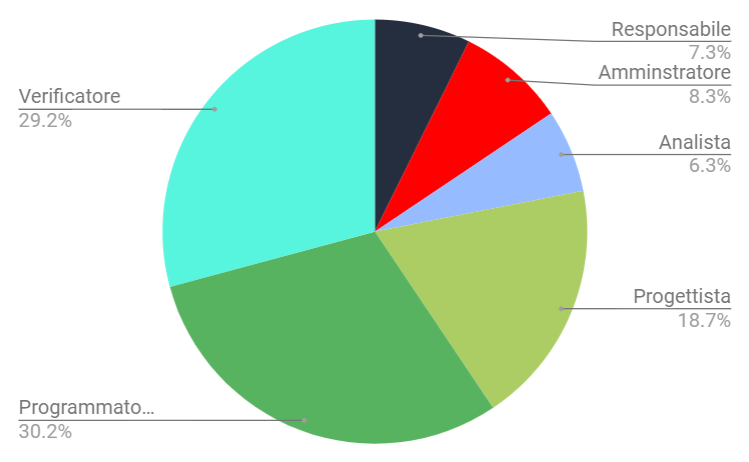
\includegraphics[width=1\textwidth]{./src/Preventivo/src/img/TortaPrevCompleto.png}  
\end{figure}
%\begin{center}
%	\begin{tikzpicture}
%		\pie[rotate = 180, color={blue, yellow, red, green, pink, orange}] {
%			7/Responsabile, % 52/723 %
%			8/Amministratore, % 59/723 %
%			4/Analista, % 29/723 %
%			20/Progettista, % 142/723 %
%			31/Programmatore, % 227/723 %
%			30/Verificatore % 218/723 %
%		}
%	\end{tikzpicture}
%\end{center}

\subsubsection{Costo complessivo}
Nella seguente tabella vengono riportati i costi complessivi delle varie fasi e infine l'importo proposto dal gruppo \Gruppo{} per la realizzazione del progetto \NomeProgetto{}:\\
{
\rowcolors{2}{\evenRowColor}{\oddRowColor}
\renewcommand{\arraystretch}{2}
\begin{longtable}{ C{5cm} C{5cm}}
\caption{Tabella del costo complessivo}\\
\rowcolor{\primaryColor}

\textcolor{\secondaryColor}{\textbf{Fase}} &
\textcolor{\secondaryColor}{\textbf{Costo \glo{fase} (in \euro{})}}\\	
\endhead

Progettazione  &  4463 \\
Sviluppo & 6046  \\
Collaudo &  2755 \\
\textbf{Totale}  &  13264 \\

\end{longtable}
}